\documentclass[brazil,hardcopy,openany,a5paper]{ufscthesis}
\usepackage[brazil]{babel}
\usepackage{amsfonts, amsmath, amsthm, amsbsy,amssymb,bm,mathtools} % For math fonts, symbols and environments %
\usepackage{graphicx} 		% Required for including images
\usepackage{transparent}	% may be required for inkscape pdf figures (http://bit.ly/18i5Oga)
\usepackage{listings}
\usepackage[abnt-emphasize=bf]{abntex2cite}
\usepackage{caption}
\usepackage{multirow}
\usepackage{lscape}
\usepackage[T1]{fontenc}
\sloppy
\usepackage{siunitx}
\usepackage{nameref}
\usepackage{float}

\newcommand{\source}[1]{\small \caption*{Fonte: {#1}} } % Criar fonte embaixo da figura

\newsubfloat{figure}		% Allow subfloats in figure environment (http://bit.ly/1C20NAj)
\graphicspath{{figures/}} 	% Location of the graphics files

\usepackage{siunitx} % units package
\let\DeclareUSUnit\DeclareSIUnit
\let\US\SI
\let\us\si
\DeclareUSUnit\inch{in}
\sisetup{detect-all}  %it may be necessary to load it after loading the font package

\citebrackets[]

%----------------------------------------------------------------------
% Comandos criados pelo usuário
\newcommand{\afazer}[1]{{\color{red}{#1}}} % Para destacar uma parte a ser trabalhada
\DeclareMathOperator*{\argmin}{\arg\!\min}
\DeclareMathOperator*{\argmax}{\arg\!\max}

%----------------------------------------------------------------------
% Identificadores do trabalho
% Usados para preencher os elementos pré-textuais
\instituicao[a]{Universidade Federal de Santa Catarina} % Opcional
\departamento[a]{Biblioteca Universitária}
\programa[o]{Programa de Pós-Graduação em Engenharia Civil} 
\curso{Engenharia de Engenharia Civil}
\documento[a]{Dissertação} % [o] para dissertação e trabalho de conclusão de curso [a] para tese
\grau{Mestre} % doutor, mestre, engenheiro, etc.
\titulo{PREDIÇÃO DE CONFORTO TÉRMICO EM ESCRITÓRIOS VENTILADOS NATURALMENTE POR MEIO DE REDES NEURAIS ARTIFICIAIS}
\subtitulo{} % Opcional
\autor{Marcelo Salles Olinger}
\local{Florianópolis} % Opcional (Florianópolis é o padrão)
\data{28}{Fevereiro}{2019}
\orientador[Universidade Federal de Santa Catarina]{Profa. Ana Paula Melo, Dra.}

\begin{document}
	
	\frontmatter
	\folhaderosto[]%pre/Ficha_Catalografica.pdf]
	
	\mainmatter

	\chapter{Introdução}
	\label{chapter:introducao}
	
	A demanda de energia para o resfriamento de ar em edificações mais que triplicou do ano de 1990 a 2016. De acordo com a Agência Internacional de Energia (IEA, 2018), o consumo de energia elétrica global destinado ao resfriamento de edificações em 2016 foi de 2.020 TWh/ano, correspondendo a quase um quinto do consumo total no setor. Se não houver mudanças no cenário atual, estima-se que a demanda por energia para resfriamento mais que triplicará até o ano de 2050, representando 37\% do aumento no consumo de eletricidade em edificações. Isso corresponderá a 11,5\% do consumo de energia total em edificações comerciais. Esse cenário é ainda mais impactante em países de clima quente, com economias emergentes. Das 2,8 bilhões de pessoas que vivem nas partes mais quentes do mundo hoje, apenas 8\% possui condicionamento de ar para resfriamento. No Brasil, a parcela do resfriamento de ar nas cargas de pico das redes elétricas em 2016 correspondia a 7,6\% do total. Até o ano de 2050, essa parcela pode representar 30,8\% da carga de pico, se nenhuma medida for tomada para a mitigação do problema.
	
	O crescimento econômico e populacional aumentam a demanda de energia. Essa demanda pode causar grandes impactos ambientais, como poluição, alterações climáticas e esgotamento dos recursos naturais. Para garantir a melhora na qualidade de vida de forma sustentável, busca-se políticas de incentivo à eficiência energética. No Brasil, desde 2009 o INMETRO possui um programa de etiquetagem de edificações voltado para padrões de eficiência energética de edificações (BRASIL, 2009).
	
	A redução dos impactos ambientais relacionados ao resfriamento de edificações pode ser alcançada através da geração de energia proveniente de fontes renováveis, do desenvolvimento de equipamentos com maior eficiência energética, ou pela busca de soluções passivas. O resfriamento passivo é um conjunto de técnicas sustentáveis para resfriar edifícios por meios naturais (SAMANI et al., 2016). Consiste em qualquer sistema que busca minimizar, ou eliminar se possível, o uso de sistemas de condicionamento de ar. Técnicas de resfriamento passivo têm o objetivo de reduzir as altas temperaturas internas e o consumo de energia para resfriamento, proporcionando conforto térmico para os ocupantes.
	
	Uma das técnicas de resfriamento passivo é a ventilação natural (VN). A VN como estratégia para resfriamento de edificações é um dos componentes fundamentais no desenho de edifícios energeticamente eficientes. Técnicas de VN são encontradas ao longo de toda a história, e hoje vêm sendo atualizadas de acordo com novos estudos no campo de conforto térmico e desenhos sustentáveis de edificações (PESIC; CALZADA; ALCOJOR, 2018). Além de assegurar a qualidade do ar, a ventilação natural promove o resfriamento da edificação, proporcionando conforto térmico aos usuários quando as condições do clima externo são favoráveis (YAO et al., 2009).
	
	Para que o conforto térmico dos usuários seja garantido sem um consumo significativo de energia, é importante entender como ocorrem as variações térmicas em um edifício antes de construí-lo. Análises durante os estágios iniciais de projeto de uma edificação com VN podem apontar decisões fundamentais para o desempenho térmico. No estágio inicial de projeto, o potencial de otimização é maior e nesta etapa qualquer estimativa da influência dos ocupantes no conforto e desempenho energético pode fazer diferença nas tomadas de decisão (BELLERI; LOLLINI; DUTTON, 2014; ROETZEL; TSANGRASSOULIS; DIETRICH, 2014).
	
	Atualmente, a forma mais avançada de predição do desempenho energético de edificações é a simulação computacional. Porém, simulações energéticas dinâmicas requerem modelos detalhados e enfrentam diversos problemas associados principalmente a informações necessárias para dados de entrada do modelo processado (CORGNATI et al., 2013). Através do uso de metamodelos, é possível obter resultados próximos aos de simulações de desempenho energético complexas, facilitando sua aplicação em diversas áreas.
	
	Metamodelos para eficiência energética de edificações podem ser desenvolvidos a partir de diversos métodos (ØSTERGÅRD; JENSEN; MAAGAARD, 2018). A solução mais apropriada depende do contexto e propósitos de cada aplicação. O desenvolvimento de um metamodelo capaz de estimar conforto térmico em edificações comerciais já foi proposto por Rackes, Melo e Lamberts (2016). Voltado principalmente a tipologias de escolas, o metamodelo estima a fração de horas de ocupação em que os ocupantes sentiriam desconforto por calor ao longo do ano, através do modelo de máquina de vetores de suporte.
	
	A avaliação do potencial de resfriamento por VN em edificações apresenta desafios, por apresentar comportamentos complexos e fazer-se necessária desde a fase inicial de projeto. Por meio de ferramentas de aprendizagem automática, surge a possibilidade do desenvolvimento de metamodelos capazes de obter resultados de conforto térmico em edificações de forma simples e rápida. 
	
	
	\section{Objetivos}
		\subsection{Objetivo geral}

	O objetivo deste estudo é desenvolver um metamodelo por meio de rede neural artificial, capaz de estimar o conforto térmico em edifícios de escritórios ventilados naturalmente.
	
		\subsection{Objetivos específicos}
	
	Dentre os objetivos específicos deste trabalho estão:

		\begin{itemize}
			\item identificar o universo de possíveis características encontradas em edifícios de escritórios ventilados naturalmente no Brasil;
			\item definir as variáveis mais influentes no desempenho térmico dos edifícios ventilados naturalmente, e as variáveis pouco influentes;
			\item explorar formas de simplificar um modelo de edifícios para que possa ser representado com apenas uma zona térmica.
		\end{itemize}
	
	\chapter{Metodologia}
		\label{chapter:metodologia}

		\section{Banco de Dados de Edificações de Escritórios}
		
		A partir do banco de dados de edificações de escritórios com VN disponibilizado por Pereira e Neves (2018), serão levantadas possíveis configurações a se considerar nos modelos utilizados para compor a base dados de simulações para o desenvolvimento do metamodelo.
		
		Dentre as informações disponíveis no banco de dados, obtém-se: áreas, dimensões, formato e número de pavimentos das edificações; cores das paredes externas e coberturas; dimensões das salas; informações relacionadas à distribuição das aberturas nas fachadas; características das janelas referentes à geometria, abertura efetiva e tipo de vidro.
		
		Serão observadas as faixas de valores dos parâmetros, assim como as suas distribuições de ocorrências. Assim, os modelos gerados posteriormente para as simulações termoenergéticas estarão de acordo com o que é construído na prática.
		
		Como as edificações do banco de dados localizam-se na cidade de São Paulo, esse será o clima para qual o metamodelo será desenvolvido.
		
		\section{Conforto Térmico}
		
		A variável de saída do metamodelo a ser desenvolvido é a fração de horas de desconforto por calor. Neste trabalho, o indicador escolhido para o limite superior da temperatura será estabelecido pelo método de conforto adaptativo da ASHRAE Standard 55 (2017), para 80\% de satisfação entre os ocupantes.
		
		Durante as simulações, para cada timestep em que haja ocupação na sala, será calculado se a temperatura operativa da zona térmica ultrapassa o limite superior determinado pelo método adaptativo da ASHRAE Standard 55 (2017). Ao fim de cada simulação, será obtido a fração de horas de desconforto para cada zona térmica modelada, de acordo com a Equação \ref{eq:FHD}:
		
		\begin{equation}
		\label{eq:FHD}
		FHD = \frac{\sum{timestep_{sup}}}{\sum{timestep_{ocup}}}
		\end{equation}
		
		Onde:
		
		$FHD$ é igual a fração de horas de desconforto por calor na zona térmica;
		
		$\sum{timestep_{sup}}$ é igual ao somatório dos timesteps em que há ocupação da zona térmica e a temperatura operativa ultrapassa o limite superior determinado pelo método adaptativo;
		
		$\sum{timestep_{ocup}}$ é igual ao somatório dos timesteps em que há ocupação da zona térmica.
		
		Na aplicação do metamodelo, será possível considerar a velocidade do ar, que aumenta o limite superior da faixa de conforto. O propósito ao se considerar a velocidade do ar é avaliar o potencial de uso para ventiladores.		
		
		Como o modelo de ventilação natural do programa EnergyPlus não calcula a velocidade do ar dentro das zonas, a consideração será aplicada após as simulações, no momento da avaliação do conforto em cada timestep. A consideração da velocidade do ar será realizada de acordo com a Equação \ref{eq:Tsup}.
		
		\begin{equation}
		\label{eq:Tsup}
		T_{sup} = T_{sup,0} + T_{v_{ar}}
		\end{equation}
		
		Onde:
		
		$T_{sup}$ é igual à temperatura limite superior na faixa de conforto, considerando-se a velocidade do ar;
		
		$T_{sup,0}$ é igual à temperatura limite superior na faixa de conforto definida pelo método adaptativo;
		
		$T_{v_{ar}}$ é igual à margem extra de temperatura permitida pela consideração da velocidade do ar.
		
		Quando utilizado o método de conforto adaptativo da ASHRAE Standard 55 (2007), o aumento no limite superior de temperatura em relação à velocidade do ar é baseado na Tabela \ref{table:var}.		
		
		\begin{table}[!h]
			\centering
			\caption{Aumento nos limites de aceitabilidade de temperatura operativa em ambientes naturalmente condicionados controlados pelo usuário.}
			\label{table:var}
			\begin{tabular}{|c |c |}
				\hline
				\textbf{Velocidade média do ar} & \textbf{Temperatura} \\
				\hline
				0,6 m/s & 1,2 K \\
				\hline
				0,9 m/s & 1,8 K \\
				\hline
				1,2 m/s & 2,2 K \\
				\hline 
			\end{tabular}
			\begin{flushleft}
			Fonte: ASHRAE Standard 55 (2017)
			\end{flushleft}				
		\end{table}
	
		Baseando-se nos valores da Tabela \ref{table:var}, serão consideradas estas três possibilidades, além do valor igual a zero, caso o uso de ventilador não seja considerado.
		
		\section{Modelo Preliminar}
		
		Sabendo-se que o metamodelo irá predizer o conforto térmico baseado no método adaptativo da ASHRAE Standard 55 (2017), o principal dado de saída a se obter nas simulações é a temperatura operativa da zona térmica, assim como a temperatura do ar externo. Portanto, todo o desenvolvimento dos modelos do trabalho será voltado para que se obtenha, com boa precisão, a temperatura operativa das zonas térmicas e, posteriormente, a sua relação com a temperatura do ar externo, chegando-se ao indicador de conforto térmico.
		
		Inicialmente serão consideradas as características observadas no banco de dados de Pereira e Neves (2018). Porém, há certas informações que não estão disponibilizadas pelo banco de dados analisado, como as relacionadas às propriedades termofísicas dos materiais da envoltória, às cargas térmicas dos equipamentos, ou aos padrões de ocupação. Esses parâmetros serão considerados a partir do que é proposto pela INI-C (2018). A Tabela \ref{table:parametros} apresenta os parâmetros que serão considerados no desenvolvimento dos modelos, com suas faixas de valores admitidos.	
		
		\begin{table}[!h]
			\centering
			\caption{Parâmetros considerados e variação nos valores.}
			\label{table:parametros}
			\begin{tabular}{|l |r |}
				\hline
				\textbf{Parâmetro} & \textbf{Valores admitidos} \\
				\hline
				Largura da edificação & 7,5 - 60 [m] \\
				\hline
				Razão entre largura e profundidade & 0,25 - 4 [-] \\
				\hline
				Número de pavimentos & 1 - 20 [-] \\
				\hline 
				Azimute do eixo principal & 0 - 359 [$^{\circ}$] \\
				\hline 
				Pé-direito & 2,5 - 4 [m] \\
				\hline 
				Percentual de abertura da fachada & 0,1 - 09 [-] \\
				\hline 
				Fator de abertura da janela & 0,1 - 1 [-] \\
				\hline 
				Fator solar do vidro & 0,35 - 0,87 [-] \\
				\hline 
				Transmitância da parede & 0,51 - 4,84 [W/m$^2$K] \\
				\hline 
				Capacidade térmica da parede & 20 - 290 [kJ/m$^2$K] \\
				\hline 
				Absortância da parede & 0,2 - 0,9 [-] \\
				\hline 
				Sombreamento & 0 - 50 [$^{\circ}$] \\
				\hline 
				Densidade de ocupação & 0,01 - 1,00 [pessoas/m$^2$] \\
				\hline 
			\end{tabular}
			\begin{flushleft}
				Fonte: o autor.
			\end{flushleft}				
		\end{table}

		A base de dados será desenvolvida a partir de simulações termo-energéticas realizadas através do programa de simulação computacional EnergyPlus 8.9 (DOE, 2018). Os modelos simulados serão obtidos a partir da parametrização de uma tipologia base, que terá diversos parâmetros variados pelo método de amostragem do hipercubo latino (abordado no item 3.6). Cada modelo obtido representará um pavimento de uma edificação com seis salas de escritórios, onde cada sala representará uma zona térmica (Figura \ref{fig:croqui}). O corredor será modelado com duas janelas, uma em cada extremidade.
		
		\begin{figure}[h]
			\centering
			\caption{Croqui da tipologia base}
			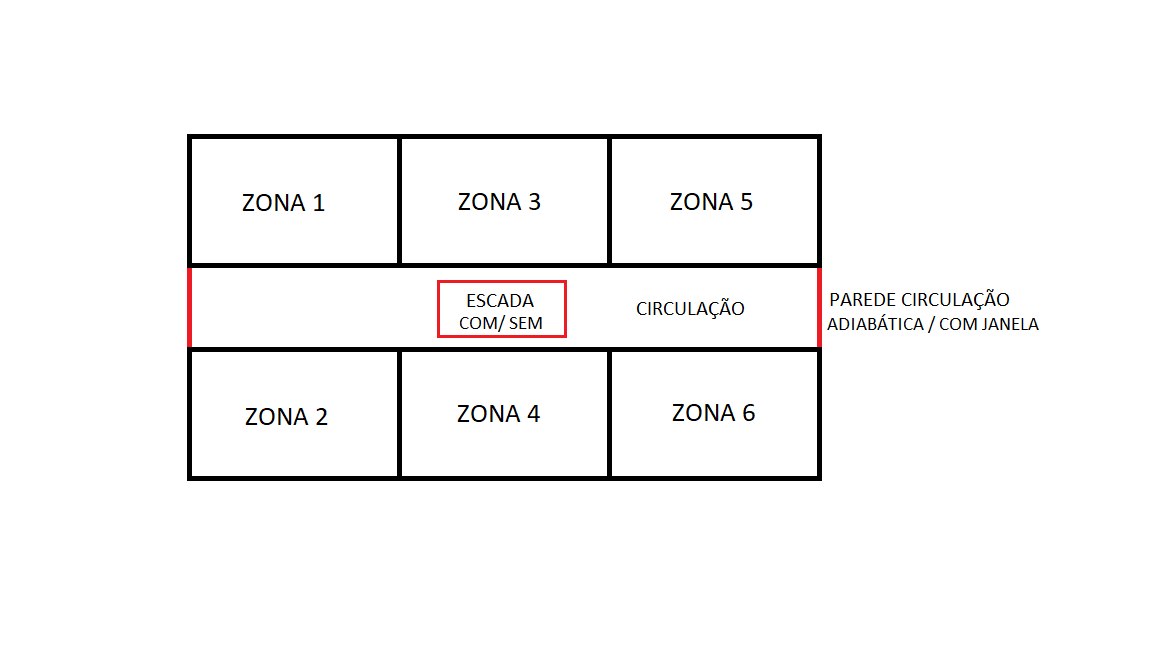
\includegraphics[width=1\linewidth]{img/CROQUI.png}
			\label{fig:croqui}
		\end{figure}
		\begin{flushleft}
			Fonte: o autor.
		\end{flushleft}
		
		Devido a limitações na obtenção dos coeficientes de pressão para as faces externas da edificação, as edificações modeladas terão sempre formato retangular.
		
		A partir dessa tipologia, serão definidas diferentes proporções geométricas, levando-se em consideração a largura, profundidade, altura da edificação e o pé-direito. Também serão parametrizados a altura do pavimento e a orientação da edificação.
		
		As aberturas do modelo também serão variadas. Cada sala terá uma porta. Salas com apenas uma fachada, possuirão uma janela; salas com duas fachadas poderão possuir uma ou duas janelas. As janelas modeladas possuirão diferentes frações de abertura para representar diferentes modelos de janela tipicamente encontrados nas edificações de escritórios. As dimensões das janelas também serão variadas. Além da área da abertura ter influência direta nas trocas de ar das zonas, a altura também pode ter influência devido à força de empuxo causada pelas diferenças de densidade do ar. Devido a isso, a altura da janela também será variada. Para o vidro das janelas, diferentes materiais serão utilizados, variando-se sua transmitância e fator solar.
		
		A variação nas propriedades termofísicas da envoltória representará diferentes materiais construtivos, possibilitando a descrição de uma quantidade significativa do universo de casos aplicáveis às edificações de escritórios consideradas. Serão variadas a transmitância térmica, capacidade térmica e absortância. Os pisos e as lajes entre pavimentos serão considerados como lajes de concreto com piso cerâmico, com as propriedades térmicas apresentadas na Tabela 3.3. As coberturas serão modeladas como laje de cimento e telhado de fibrocimento, separadas por uma câmara de ar. As propriedades térmicas da cobertura também estão apresentadas na Tabela 3.3. Como apenas um pavimento é modelado, pisos e tetos de pavimentos intermediários são considerados adiabáticos.
		
		\section{Ventilação natural}
		
		A ventilação natural será modelada a partir do modelo AirflowNetwork (AFN) do EnergyPlus (DOE, 2018).
		
		O controle das janelas será estabelecido pela diferença de temperatura entre o ar externo e o ar da zona. As trocas de ar nas portas ocorrerão apenas por frestas, por considerar-se que portas de escritórios não ficam abertas normalmente.
		
		Os coeficientes de pressão nos nós externos à edificação serão definidos através da base de dados de Tokyo (TPU, 2018), e para cada janela será utilizado o valor médio dos pontos disponíveis para sua área na fachada, de acordo com a Figura X.
		
		\section{Modelo simplificado}
		
		O objetivo de gerar um modelo de RNA para se obter o EHF faz com que se busque parametrizar ao máximo os modelos desenvolvidos no Energyplus. Essa parametrização pode facilitar o desenvolvimento de amostras para a pesquisa, assim como garantir uma relação mais direta dos parâmetros de entrada com os dados de saída. Portanto, nesta etapa do método busca-se simplificar e parametrizar o modelo de escritório desenvolvido no Energyplus, atentando-se às limitações relacionadas à simplificação do modelo.
		
		Dentre as simplificações consideradas, estão:
		
		\begin{itemize}
		\item cálculo do Cp através do método analítico, em vez dos dados obtido por medições em túnel de vento pela TPU;
		\item representação dos materiais da envoltória através de duas camadas: uma camada representando a capacidade térmica (concreto), e uma camada para regular a transmitância (objeto Material:NoMass);
		\item modelagem da zona que representa um escritório isoladamente, sem modelar as demais zonas térmicas da edificação. Para isso, são definidas as condições de contorno relacionadas às faces da zona correspondentes a paredes adjacentes à edificação;
		\item definição de um coeficiente de infiltração relacionado à infiltração de ar pela porta, e do valor de Cp relacionado à porta, que está voltada para o corredor, e não para o ambiente externo.`
		\end{itemize}
		
		O impacto nos resultados das simulações serão verificados para cada uma das simplificações mencionadas. Desta forma, será definida a forma mais adequada de simplificar o modelo, assim como a margem de erro que espera-se encontrar ao assumir tais simplificações.
		
		\section{Túnel de vento x Método analítico}
		
		Para verificar o quanto os resultados das simulações são influenciados pela fonte utilizada na definição dos valores de Cp, comparou-se os resultados de ACH e EHF em simulações com valores de Cp obtidos pela base da TPU aos resultados obtidos para simulações com valores de Cp obtidos pelo método analítcio de SwamiShandra(?), que é algoritmo padrão do Energyplus.
		
		Equanto valores de Cp através do método analítco podem ser obtidos pra quaisquer razões entre dimensões das fachadas da edificação, os valores da base TPU são fornecido para edificações com geometrias específicas. Ambas as fontes são limitadas a edificações retangulares.
		
		Para o tipo de edificação simulados neste estudo, a TPU disponibiliza valores de Cp para 25 geometrias diferentes, das quais 13 são para edificações altas (highrise), e 12 são para edificações baixas (lowrise). Para cada uma dessas geometrias disponíveis, valores de Cp são disponibilizados para diversos pontos na fachada da edificação, de acordo com a Figura X.
		
		Para verificar as diferenças nos valores de Cp, calculou-se valores de Cp correspondentes a cada geometria disponível pela TPU através do método analítico, e subtraiu-se o valor de Cp calculado para cada fachada pelos valores disponibilizados pela base da TPU para a fachada correspondente (Equação X).
		
		A partir dessas diferenças entre os valores de Cp, escolheu-se a geometria com a maior média de diferença absoluta para se analisar a influência da diferença desses valores nos resultados das simulações no Energyplus.
		
		O modelo base para verificar as diferenças dos resultados utilizando-se valores de Cp com origens diferentes foi o modelo de pavimento com 6 escritórios. Para evitar a influência do solo e da cobertura, considerou-se um pavimento intermediário. A base da TPU permite a obtenção de diferentes coeficientes de pressão para diferentes janelas, como mencionado na seção anterior. No modelo baseado no método analítico, utilizou-se um valor de Cp por fachada, devido à limitação do método. Uma amostra de 1000 casos foi gerada pelo método de amostragem do hipercubo latino. A amostra gerada teve parâmetros variados de acordo com a Tabela \ref{table:cpmethod}.
		
		\begin{table}[h]
			\centering
			\caption{Descrição da tabela.}
			\label{table:cpmethod}
			\begin{tabular}{|c |c |c |c |}
				\hline
				\textbf{Parâmetro} & \textbf{Unidade} & \textbf{Mínimo} & \textbf{Máximo} \\
				\hline
				Área & m$^2$ & 20 & 100 \\
				\hline
				Pé-direito & m & 2,4 & 3,2 \\
				\hline
				Azimute & graus & 0 & 359,9 \\
				\hline 
				Transmitância & W/m$^2$ & 0,5 & 4,4 \\
				\hline 
				PAF & - & 0,1 & 0,6 \\
				\hline 
				Ocupação & pessoa/m$^2$ & 0,05 & 0,50 \\
				\hline 
				Pavimento & - & 1 & 8 \\
				\hline 
			\end{tabular}
			\begin{flushleft}
				Fonte: ASHRAE Standard 55 (2017)
			\end{flushleft}				
		\end{table}
				
		Para cada caso da amostra, foram simulados um modelo com Cp’s baseados no método analítico, e um modelo com Cp’s baseados na base da TPU (túnel de vento).
		
		\section{Representação da envoltória}
		
		Para possibilitar a parametrização contínua e independente das propriedades termofísicas da envoltória, considerou-se a utilização de uma parede com propriedades equivalentes, modelada com uma camada de concreto, para representar a capacidade térmica, e uma camada modelada com o objeto Material:NoMass, para regular a transmitância.
		A validação da modelagem simplificada da parede foi feita para 3 tipos de parede:
		
		\begin{itemize}
			\item parede de concreto;
			\item parede de alvenaria e reboco;
			\item parede de gesso com lã de rocha.
		\end{itemize}`
		
		Como a modelagem da parede de alvenaria possui uma camada de ar no meio da parede, considerou-se a possibilidade de a capacidade térmica a ser considerada na parede de concreto+eps ser melhor representada considerando-se apenas metade da parede.
		
		Para validar essa simplificação, gerou-se uma amostra utilizando HCL, com 100 casos. O modelo preliminar sofreu variação dos seguintes parâmetros: área, razão entre largura e profundidade da zona, pé-direito, azimute, absortância, PAF, taxa de ocupação.
		
		Cada caso da amostra foi simulado com os três tipos de paredes diferentes, e suas paredes equivalentes. No caso da parede de alvenaria, um modelo de parede equivalente foi desenvolvido considerando-se apenas metade da parede de alvenaria.
		
		A partir dos resultados, observou-se a diferença média entre as temperaturas operativas das zonas nos modelos com as paredes referências em relação aos modelos com as respectivas paredes equivalentes. O mesmo foi feito comparando-se o EHF.
		
		\section{Condição de contorno das paredes adjacentes}
		
		Simular apenas uma zona, em vez de um edifício ou de um pavimento com diversas zonas, possibilita a simulação de muitos casos diversos em menos tempo.
		
		Para modelar apenas uma zona, considerou-se as paredes correspondentes a superfícies voltadas para outros escritórios como adiabáticas. A superfície que representa a parede voltada para o corredor foi testada com duas condições de contorno: como adiabática, e como outdoors, sem incidência de vento ou sol.
		
		O modelo de referência é o modelo preliminar. Para cada caso referência, seis modelos de uma zona foram modelados, correspondendo a cada uma das zonas do modelo referência. A modelagem da ventilação natural sofre um impacto significativo quando o escritório é modelado como apenas uma zona. Esse impacto é devido à forma como a rede de fluxo de ar é montada. No caso do modelo referência, a porta é voltada para o corredor, enquanto que no caso de uma única zona, a porta da zona é voltada para a rua. Além disso, não é possível modelar uma porta em uma parede adiabática. Para não deixar a diferença na ventilação natural influenciar as análises comparativas entre os modelos, a ventilação natural não foi modelada para esta etapa. Em vez disso, os modelos foram desenvolvidos com uma taxa de infiltração de ar constante durante a ocupação. O valor escolhido para a taxa de renovação de ar foi igual ao valor médio obtido na etapa da comparação entre os métodos de obtenção dos valores de Cp, que é igual a 30 ach.
		
		Para validar o uso de diferentes condições de contorno, comparou-se os resultados de EHF e temperaturas operativas das zonas únicas com os modelos referência. A condição de contorno com menores diferenças médias absolutas, foi escolhida para gerar o modelo simplificado.
		
		\section{Modelagem da ventilação natural no modelo simplificado}
		
		A modelagem da ventilação natural no modelo simplificado deve ser adaptada para se ter resultados correspondentes ao esperado em relação aos modelos referência.
		
		No AFN do EnergyPlus não é possível modelar aberturas ou infiltração de ar em superfícies adiabáticas. Para contornar esse problema, no caso de se modelar uma parede voltada para o corredor como adiabática, é possível associar a infiltração referente à porta a uma outra superfície da zona que esteja voltada para o ambiente externo. A solução para isso é modelar diretamente os objetos dos nós relacionados às aberturas dos modelos, ou seja, os coeficientes de pressão. Desta forma é possível definir valores de Cp para superfícies (seja janela ou parede) considerando-se qualquer orientação desejada, e não necessariamente a orientação definida para aquela superfície na geometria do modelo.
		
		A modelagem do fluxo de ar pelas portas dos escritórios nos modelos de zona única foi desenvolvida com o objeto AirflowNetwork:MultiZone:Surface:Crack. O motivo para se utilizar este objeto é porque este é um objeto que pode ser associado a qualquer superfície. Portanto, o objeto crack é associado à parede externa oposta à parede voltada para o corredor.
		
		Esta forma de contornar o problema da infiltração na parede adiabática impede que os valores de Cp sejam calculados automaticamente pelo Energyplus, portanto valores de Cp específicos são calculados para cada abertura do modelo. A fórmula utilizada para calcular os valores de Cp é a mesma do algoritmo padrão do Energyplus, porém a orientação da abertura é alterada conforme desejado.
		
		Além da solução descrita para atribuir adequadamente os valores de Cp às aberturas, existe outra limitação: as diferenças de pressão entre as zonas dos escritórios e do corredor variam de acordo com a direção do vento, mas não de forma igual ao que se calcularia considerando-se o Cp da fachada. Dentro da rede de fluxo do AFN, a pressão do corredor depende das trocas de ar entre todas as zonas adjacentes e as trocas de ar pelas janelas do corredor. Em um modelo de zona única isso não poderia ser incluído. Para tentar contornar este problema, buscou-se uma forma de gerar um Cp equivalente para a porta no modelo de uma única zona. Esse cálculo foi feito considerando-se a equação X. A equação proposta leva em conta as resistências de todas as aberturas da edificação de referência, e calcula uma relação entre as pressões do ar externo e do corredor para cada direção de vento. Essas relações entre as pressões são adotadas então como valores de Cp.
		
		Devido a essas considerações, a validação foi conduzida para duas condições: considerando-se o Cp calculado diretamente pelo método analítico, e considerando-se o Cp equivalente, que leva em conta a relação entre as pressões nas zonas para cada direção de vento.
		
		Estas análises foram conduzidas considerando-se diferentes valores de coeficiente de infiltração para o objeto AirflowNetwork:MultiZone:Surface:Crack, para ajustar o valor mais adequado à taxa de infiltração que se obtém no modelo referência.
		
		%Como as taxas de infiltração são influenciadas pela temperatura do ar, as comparações com os modelos referências foram feitas considerando-se diferentes faixas de temperatura.
		
		\section{Análise de sensibilidade}
		
		Com a definição de como serão gerados os modelos simplificados, uma análise de sensibilidade será aplicada. Através da análise de sensibilidade, a influência das diferentes variáveis nos modelos serão avaliadas. Características parametrizáveis nos modelos preliminares que não sejam relevantes nos resultados de temperatura operativa e, consequentemente, fração de horas de desconforto por calor, serão fixadas.
		
		O método de Sobol (1993) será utilizado para a análise de sensibilidade, pois permite a identificação de parâmetros influentes, mesmo para casos onde a relação entre as entradas e saídas dos modelos são não-monotônicas  e apresentam efeitos colineares. A amostragem para essa análise é definida pelo próprio método. A aplicação será feita através da biblioteca SALib (HERMAN; USHER, 2017), escrita na linguagem Python (PYTHON, 2018). A partir de uma amostra com 99.978 casos, obteve-se índices de sensibilidade para análise de 1ª ordem, 2ª ordem, e total.
		
		\section{Desenvolvimento da rede neural artificial}
		
		A base de dados utilizada para o treinamento do metamodelo foi desenvolvida a partir de XXX.XXX resultados de simulações, amostrados pelo método de amostragem de Sobol. A etapa de validação foi executada com outra amostra de XX.XXX casos, amostrados pelo método do HCL. Na amostra da validação, os parâmetros não incluídos como dados de entrada para a RNA tiveram os valores fixados iguais aos da amostra utilizada para o treinamento. O motivo para se utilizar diferentes métodos de amostragem é para evitar qualquer enviesamento possivelmente relacionado ao método de amostragem.
		
		Após a etapa de validação, a amostra gerada para a AS foi utilizada para verificar o desempenho da RNA quando os valores dos parâmetros não considerados como dados de entrada da RNA variam. A escolha desta 
		
		Após definir quais variáveis do modelo preliminar exigem parametrização, e quais podem ser fixadas, a configuração do modelo base final será definida.
		
		A partir do modelo base final, será desenvolvida uma base de dados através do método de amostragem do Hipercubo Latino.
		
		É importante ressaltar que cada modelo simulado pelo EnergyPlus possuirá diversas zonas térmicas, e que cada zona será considerada como um caso específico para a base de dados utilizada no treinamento da rede neural artificial (RNA). Portanto, cada caso do banco de dados gerado para o treinamento da RNA será um vetor, contendo diversas informações sobre as características da sala, e dos resultados obtidos de fração de horas de calor para esta sala.
		
		O desenvolvimento do metamodelo será por meio do sistema computacional de redes neurais artificiais. Esse processo será executado através da linguagem de programação Python. A RNA será treinada com 80\% da base de dados gerada. A parte restante será utilizada para validação do metamodelo.
		
		A forma como as variáveis descritas nos modelos simulados serão introduzidas no metamodelo a ser desenvolvido podem influenciar a precisão e a representação adequada dos fenômenos termofísicos. No processo de definição das variáveis de entrada do metamodelo, busca-se a melhor forma de descrever as diversas características das salas e do clima. Esse é um processo iterativo, no qual varia-se diferentes variáveis de entrada, utilizando-se às vezes transformações, normalizações e funções destas. É importante também observar os hiper-parâmetros (parâmetros relacionados ao processo de aprendizagem automática) escolhidos na criação da RNA. A precisão da rede pode depender do número de nós, número de camadas, assim como outros parâmetros definidos durante o processo de treinamento.
		
		Para validar a RNA, serão comparados os resultados obtidos através do metamodelo com os casos não vistos da base de dados de simulações do EnergyPlus. Como indicadores de precisão, serão utilizados a raiz quadrada da média dos erros ao quadrado (RMSE) e o coeficiente de determinação (R$^2$).
		

%\bibliographystyle{lib/abntex2-num}
%\bibliographystyle{lib/abntex2-alf}
\bibliography{citacoes}
	
\end{document}